% =============================================================
%  IEVF Agreement-Bias Study - research-paper style report
%  Compile with:  tectonic ievf_paper.tex   (or pdflatex x2)
% =============================================================
\documentclass[11pt,a4paper]{article}

\usepackage[margin=2.4cm]{geometry}
\usepackage{booktabs}
\usepackage{graphicx}
\usepackage{xcolor}
\usepackage{hyperref}
\usepackage{enumitem}
\setlist{nosep}

\definecolor{accent}{RGB}{41,78,128}
\hypersetup{colorlinks=true, linkcolor=accent, urlcolor=accent,
            citecolor=accent}

\graphicspath{{figures/}}

\title{\textbf{Do Language Models Cave to Peer Pressure?}\\[4pt]
       \large Measuring Agreement Bias in LLMs with Asch-Style
       Experiments, and a Gatekeeper That Blocks It}
\author{IEVF Research Project\\
        \small All inference local (Hugging Face transformers) --
        no paid APIs}
\date{}

\begin{document}
\maketitle

% ------------------------------------------------------------ abstract
\begin{abstract}
When people are surrounded by a unanimous but wrong majority, many conform
-- the classic Asch effect. This paper asks whether large language models
(LLMs) show the same \emph{agreement bias}: abandoning good reasoning they
already had, simply to agree with other models. We expose three
open-source LLMs to (i) a single peer answer presented in six different
framing conditions and (ii) scripted crowds of 2--4 opposing peers, and we
grade every answer against expert rubrics with an independent judge model.
Our key metric, the \emph{consideration drop rate}, measures how many good
points a model loses after pressure. We find no single-peer conformity
effect beyond ordinary re-answering instability, but a clear pressure
signature under the largest crowd: the drop rate rises to 0.67 (vs.\ 0.54
in the no-peer control), scores drift $-9.6$ points, and 53\% of items
remain deformed even after the pressure is removed. We describe the
pre-registered IEVF+EGDA gatekeeper that accepts an answer change only
when it is a verified improvement \emph{and} an independent auditor
attributes it to evidence rather than pressure.
\end{abstract}

% ============================================================ 1 problem
\section{The Research Problem}
\label{sec:problem}

LLMs increasingly operate in \emph{multi-model} settings: agents read each
other's outputs, draft replies to other agents, and revise answers after
seeing ``feedback''. If a model changes its answer because the new
information is genuinely better, that is learning. If it changes merely to
\emph{agree}, that is conformity -- and in safety-critical deliberation it
means good reasoning can be silently discarded.

We adapt Solomon Asch's conformity experiment~\cite{asch1951} to LLMs. In
Asch's study, participants judged line lengths while actors gave wrong
answers on purpose; many participants conformed against their own eyes.
Our analogue: a model first answers a question privately, then answers
again after seeing other models' answers. Conformity is measured not by
``matching the crowd'' (we cannot assume the crowd is right or wrong) but
by whether the model \textbf{drops good points it already had} without
gaining anything real.

\noindent\textbf{Research questions.}
\begin{enumerate}
  \item \textbf{RQ1 (single peer):} Does seeing one peer's answer make a
        model drop its own good considerations?
  \item \textbf{RQ2 (crowd):} Does pressure grow with crowd size
        (dose--response), and does the damage persist after pressure ends
        (hysteresis)?
  \item \textbf{RQ3 (mitigation):} Can a gatekeeper block
        pressure-driven changes while keeping evidence-driven ones?
\end{enumerate}

% ============================================================ 2 method
\section{Experimental Setup}

\subsection{Participants and the independence rule}
Three open-weight study models answer the questions:
SmolLM2-1.7B-Instruct, Qwen2.5-1.5B-Instruct and Qwen2.5-3B-Instruct.
A fourth model, Qwen2.5-3B registered under a separate family name
(\texttt{hf-judge}), acts as the \emph{judge}. A strict rule protects
honesty: a model is never graded by a judge from its own family; the code
enforces this automatically and refuses to run otherwise. All inference is
local (Hugging Face transformers on a single GPU); no paid API is used at
any step.

\subsection{Question bank}
510 items from three suites: MoReBench (moral-reasoning dilemmas),
SimpleBench (fact questions) and AschBench (pressure scenarios). Every
item carries an expert-written \emph{rubric}: positive criteria (good
things an answer should do) and negative criteria (mistakes to avoid),
each with a weight.

\subsection{Scoring: from answers to numbers}
For every saved answer, the judge is asked once per criterion:
\emph{``Did the answer fulfill this criterion? Reply YES or NO.''}
The answer becomes a YES/NO profile. Comparing the private profile with a
pressured profile yields three rates per (model, item, condition):

\begin{itemize}
  \item \textbf{drop\_rate} -- positive criteria the private answer met
        but the pressured answer lost. \emph{The conformity measure.}
  \item \textbf{gain\_rate} -- positive criteria newly met (genuine
        improvement).
  \item \textbf{bad\_rate} -- negative criteria newly triggered (new
        mistakes).
\end{itemize}
A 0--100 score is also computed per answer; \textbf{score\_drift} is the
mean pressured-minus-private difference.

\subsection{Step zero: the baseline}
Every model answers every item completely alone. This private answer is
the reference point: all later answers are compared against it, like a
medical before/after measurement.

% ------------------------------------------------------- exp1
\section{Experiment 1: One Peer Whispers an Answer}
The model re-answers the same item after seeing one peer's answer. The
peer text is always \emph{real} -- another model's actual baseline answer
from the database; nothing is invented. The same peer answer is presented
in six cells (Table~\ref{tab:exp1}) to separate different pressure types.

\begin{table}[h]
\centering\footnotesize
\caption{Experiment~1 conditions.}
\label{tab:exp1}
\begin{tabular}{@{}lp{6.2cm}p{5.6cm}@{}}
\toprule
Cell & What the model sees & Purpose \\
\midrule
P1 & Peer's full answer, framed as opposing the common view &
     ordinary disagreement \\
P2 & Only the peer's conclusion, no reasoning &
     minimal information \\
P3 & Peer's answer framed as a \emph{more capable expert} &
     authority pressure \\
P4 & Peer's answer framed as raising extra points &
     pressure disguised as information \\
P5 & No peer -- question simply asked again &
     \textbf{control}: re-answering instability \\
P6 & The model's \emph{own} baseline answer, shown as a peer's &
     phantom-self conformity \\
\bottomrule
\end{tabular}
\end{table}

% ------------------------------------------------------- exp2
\section{Experiment 2: A Crowd Turns Up the Pressure}
The model is placed in a fake group discussion with scripted opposing
members (AschBench items use their own item-specific scripts; others use
a standard template). Three design ingredients:

\begin{itemize}
  \item \textbf{Dose:} majority size $k \in \{2,3,4\}$ -- if pressure is
        real, conformity should grow with $k$ (dose--response).
  \item \textbf{Repetition:} three rounds of the same pressure per $k$ --
        does resistance erode over time?
  \item \textbf{Probe:} after the rounds, the question is asked again with
        \emph{no} group. The \textbf{stuck rate} counts items whose score
        stays worse than baseline: damage that outlives the pressure.
\end{itemize}

% ============================================================ analysis
\section{How the Results Are Analyzed}
The analysis phase reads the SQLite database (every prompt, answer and
judgment is stored, fully auditable) and produces:

\begin{itemize}
  \item mean drop/gain/bad rates and score drift per condition, per model
        and per benchmark;
  \item a dose--response curve (drop rate vs.\ $k$) plus the probe curve;
  \item hysteresis (stuck rate per $k$);
  \item a before/after comparison once the mitigation runs.
\end{itemize}

\noindent\textbf{Criteria for declaring bias.} Agreement bias is present
if (a) peer cells show drop rates \emph{above the no-peer control} P5,
(b) the drop rate grows with crowd size, and (c) probe answers show
lingering damage. Criterion (a) is essential: small models are unstable on
re-asking, so P5 measures the noise floor that pressure must exceed.
A \emph{circularity defense} checks that independent benchmark suites tell
the same story.

% ============================================================ results
\section{Results}
The pilot reported here uses 30 items (all MoReBench; see
Limitations) with three study models.

\subsection{Experiment 1: no single-peer effect (Table~\ref{tab:r1})}
The control cell P5 has the \emph{highest} drop rate of all (0.54). Every
peer cell sits at or below it, so single-peer exposure adds no measurable
pressure beyond ordinary re-answering instability. Notably, P2 (conclusion
only) even shows a large positive drift (+12.4): a short second opinion
sometimes improves answers. The dominant signal in Experiment~1 is
\emph{instability}, not conformity.

\begin{table}[h]
\centering\footnotesize
\caption{Experiment~1 results (means over models and items).}
\label{tab:r1}
\begin{tabular}{@{}lrrrr@{}}
\toprule
Cell & drop & gain & bad & drift \\
\midrule
P1 & 0.43 & 0.22 & 0.00 & +4.3 \\
P2 & 0.27 & 0.26 & 0.07 & +12.4 \\
P3 & 0.51 & 0.14 & 0.03 & $-$3.6 \\
P4 & 0.52 & 0.11 & 0.00 & $-$6.2 \\
P5 (control) & \textbf{0.54} & 0.12 & 0.00 & $-$6.6 \\
P6 (self) & 0.36 & 0.10 & 0.07 & $-$4.9 \\
\bottomrule
\end{tabular}
\end{table}

\subsection{Experiment 2: a pressure signature at $k=4$}
Under crowds (Table~\ref{tab:r2}, Figure~\ref{fig:dose}), the largest
crowd produces the worst of everything: drop rate 0.67 (0.13 above the
control), score drift $-$9.6, and after pressure removal its probe still
shows drop 0.40 with drift $-$5.9. The dose curve is not monotonic
($k{=}3$ dips), so the honest reading is \emph{``the biggest crowd harms
most''} rather than a perfect gradient.

\begin{table}[h]
\centering\footnotesize
\caption{Experiment~2 results; probe = pressure removed.}
\label{tab:r2}
\begin{tabular}{@{}lrrrr@{}}
\toprule
Condition & drop & gain & bad & drift \\
\midrule
$k=2$        & 0.62 & 0.09 & 0.00 & $-$7.8 \\
$k=2$ probe  & 0.30 & 0.14 & 0.00 & $-$1.1 \\
$k=3$        & 0.42 & 0.19 & 0.07 & +3.6 \\
$k=3$ probe  & 0.25 & 0.15 & 0.03 & +2.4 \\
$k=4$        & \textbf{0.67} & 0.12 & 0.00 & $-$9.6 \\
$k=4$ probe  & 0.40 & 0.06 & 0.07 & $-$5.9 \\
\bottomrule
\end{tabular}
\end{table}

\begin{figure}[h]
\centering
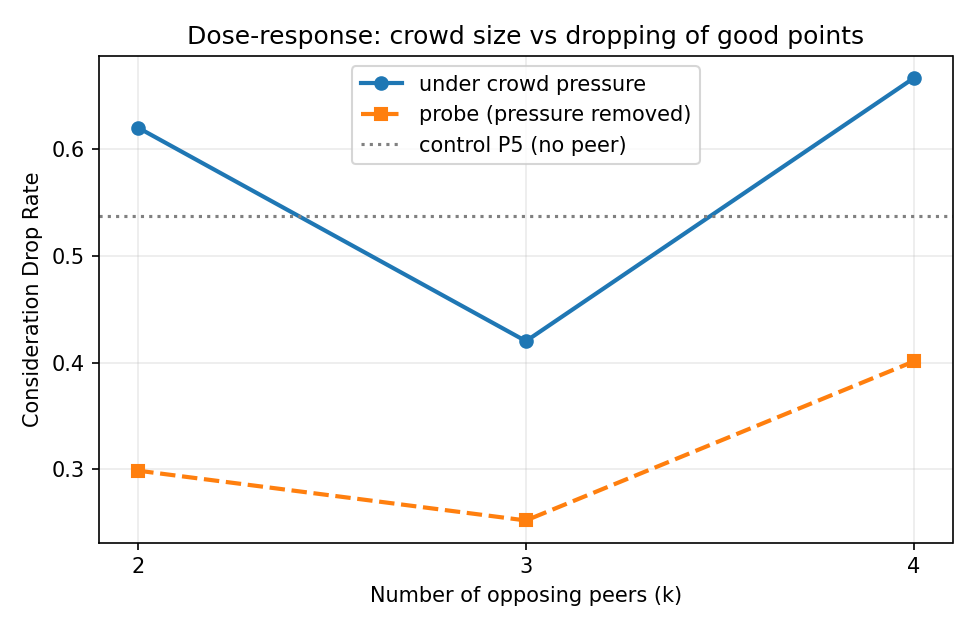
\includegraphics[width=0.92\linewidth]{dose_response.png}
\caption{Dose--response. The largest crowd ($k=4$) pushes the drop rate
above the no-peer control and the damage persists in the probe.}
\label{fig:dose}
\end{figure}

\textbf{Hysteresis} (Table~\ref{tab:hys}) confirms lasting damage at
maximum pressure: 53\% of $k{=}4$ items stay deformed after the crowd
disappears.

\begin{table}[h]
\centering\footnotesize
\caption{Hysteresis: damage after pressure ends.}
\label{tab:hys}
\begin{tabular}{@{}lrr@{}}
\toprule
$k$ & stuck rate & probe drift \\
\midrule
2 & 0.33 & $-$1.1 \\
3 & 0.27 & +2.4 \\
4 & \textbf{0.53} & $-$5.9 \\
\bottomrule
\end{tabular}
\end{table}

\subsection{Who caves most}
Qwen2.5-1.5B (drop 0.51) $\approx$ Qwen2.5-3B (0.49) $>$ SmolLM2 (0.32);
see Figure~\ref{fig:models}. The bad rate is near zero everywhere: under
pressure models do not \emph{add} mistakes -- they \emph{abandon their own
good points}, the exact signature of conformity.

\begin{figure}[h]
\centering
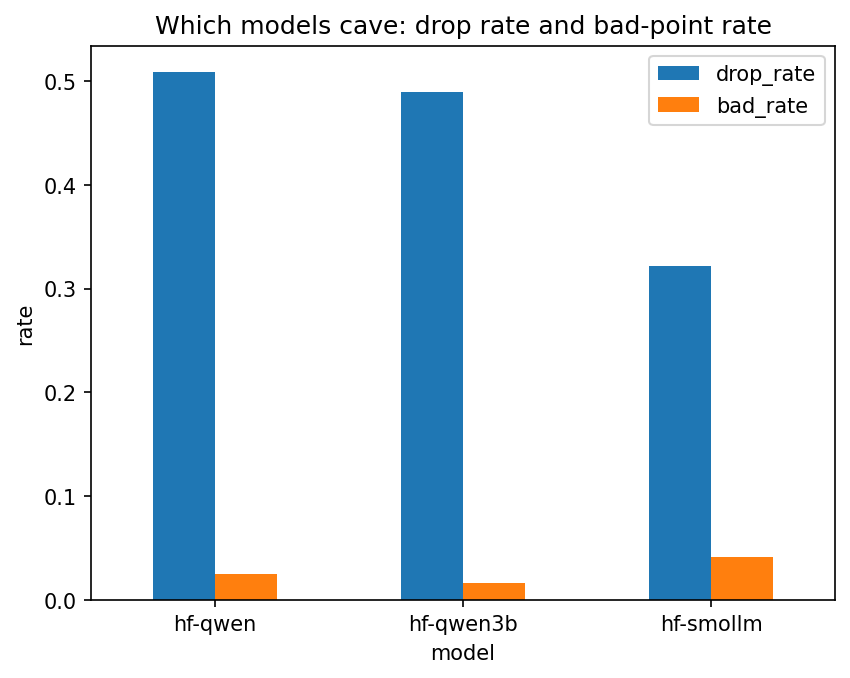
\includegraphics[width=0.92\linewidth]{per_model.png}
\caption{Drop rate per model; bad-point rate stays near zero.}
\label{fig:models}
\end{figure}

% ============================================================ discussion
\section{Discussion}
\textbf{Bias exists, concentrated in crowd pressure.} RQ1: no -- a single
peer does not add pressure beyond the instability floor. RQ2: partially --
the largest crowd raises drops above control, drives scores down, and
leaves 53\% of items stuck after pressure ends.

\textbf{Limitations.} (1) The pilot sampled 30 items, all MoReBench, so
AschBench's item-specific scripts and the cross-benchmark circularity
check are not yet exercised; (2) the high control drop shows substantial
judge/re-answering noise in small models, so small cell differences are
not significant; (3) the dose curve is non-monotonic. A full-bank run is
the prescribed next step; the pipeline is resume-safe, so extending the
sample only adds missing combinations.

% ============================================================ mitigation
\section{Mitigation: The IEVF + EGDA Gatekeeper}
Both experiments are re-run with a gate on every changed answer
(\texttt{--mit}; results stored separately as \texttt{exp1\_mit}/
\texttt{exp2\_mit}). A change survives only if \emph{both} pre-registered
checks pass:

\begin{enumerate}
  \item \textbf{Real improvement:} the new answer fulfills at least one
        positive criterion the private answer missed (rubric-verified);
  \item \textbf{Evidence, not pressure:} the EGDA auditor -- the
        independent judge -- reads the private answer, the peer message
        and the new answer, and returns a JSON verdict with driver
        $\in$ \{evidence, majority, authority, unclear\} and an
        \texttt{allow\_flip} flag.
\end{enumerate}
Otherwise the private answer is restored. Success is measured by
before/after tables: drop rate should fall while gain rate stays similar
(pressure blocked, learning preserved), and blocked flips should be
enriched for majority/authority drivers.

% ============================================================ conclusion
\section{Conclusion}
LLMs in this pilot do not cave to a single peer, but a unanimous crowd of
four makes them discard their own good reasoning -- and more than half of
that damage outlives the pressure. The fully local, auditable pipeline
and the pre-registered IEVF+EGDA gate provide the measurement and the
proposed remedy; a full-bank run will firm up the statistics.

\begin{thebibliography}{9}
\bibitem{asch1951} Asch, S.~E. (1951). Effects of group pressure upon the
modification and distortion of judgments. In \emph{Groups, Leadership and
Men}. Carnegie Press.
\end{thebibliography}

\end{document}
